\documentclass[11pt,oneside]{article}
\usepackage[paperwidth=8.25in,paperheight=11in,left=.98in,right=.98in,top=.96in,bottom=.91in,headheight=17pt,headsep=22pt,footskip=28pt]{geometry}
\usepackage[T1]{fontenc}
\usepackage[utf8]{inputenc}
\usepackage{newpxtext}
\usepackage{amsmath,amsthm,amssymb}
\usepackage{mathtools}
\usepackage{newpxmath}
\usepackage{microtype}
\renewcommand{\sfdefault}{qhv}
\usepackage{graphicx}
\usepackage{placeins}
\graphicspath{{figures/}}
\usepackage{caption}
\usepackage{tikz}
\usepackage{array,tabularx,booktabs,enumitem}
\usepackage{titlesec}
\usepackage{fancyhdr}
\usepackage{etoolbox}
\usepackage{needspace}
\usepackage{setspace}
\usepackage{hyperref}
\usepackage{bookmark}
\usepackage{url}
\usepackage{xcolor}
\usepackage[most]{tcolorbox}
\usepackage{ragged2e}
\definecolor{ink}{HTML}{352C3B}
\definecolor{bodyink}{HTML}{252A2C}
\definecolor{accent}{HTML}{70566D}
\definecolor{gold}{HTML}{A98D5E}
\definecolor{muted}{HTML}{68656B}
\definecolor{pale}{HTML}{F7F5F7}
\definecolor{rulecolor}{HTML}{DCD7DD}
\definecolor{coverink}{HTML}{282331}
\definecolor{forest}{HTML}{70566D}
\definecolor{warm}{HTML}{A98D5E}
\color{bodyink}
\newcommand{\displayface}{\fontfamily{EBGaramond-LF}\fontseries{m}\fontshape{n}\selectfont}
\newcommand{\booklabel}[1]{{\sffamily\fontsize{8}{11}\selectfont\textls[110]{\MakeUppercase{#1}}}}
\hypersetup{colorlinks=true,linkcolor=ink,citecolor=accent,urlcolor=accent,
 pdftitle={The Komorebi Methodology},pdfauthor={Komorebi P.},
 pdfsubject={Realization Calculus / Methodological Essay},bookmarksopen=true,
 bookmarksopenlevel=0,bookmarksdepth=2,pdfdisplaydoctitle=true,pdfstartview=FitH}
\setcounter{tocdepth}{1}
\setcounter{secnumdepth}{1}
\setlength{\parindent}{0pt}
\setlength{\parskip}{5.5pt plus 1pt minus .5pt}
\linespread{1.05}
\emergencystretch=2.5em
\clubpenalty=10000
\widowpenalty=10000
\raggedbottom
\Urlmuskip=0mu plus 3mu\relax
\setlist[itemize]{leftmargin=1.3em,itemsep=3pt,topsep=5pt,parsep=0em}
\setlist[enumerate]{leftmargin=1.6em,itemsep=4pt,topsep=6pt,parsep=0em}
\renewcommand\labelitemi{\textcolor{accent}{\raisebox{.17ex}{\tiny$\bullet$}}}
\titleformat{\section}{\displayface\fontsize{27}{30}\selectfont\color{ink}\raggedright}{\sffamily\fontsize{10}{13}\selectfont\color{accent}\thesection}{.65em}{}[\vspace{1pt}{\color{gold}\rule{39pt}{.75pt}}]
\titlespacing*{\section}{0pt}{21pt plus 2pt minus 1pt}{15pt}
\titleformat{name=\section,numberless}{\displayface\fontsize{27}{30}\selectfont\color{ink}\raggedright}{}{0pt}{}[\vspace{1pt}{\color{gold}\rule{39pt}{.75pt}}]
\titleformat{\subsection}{\normalfont\fontsize{12}{16}\selectfont\bfseries\color{ink}}{}{0pt}{}
\titlespacing*{\subsection}{0pt}{15pt plus 2pt minus 1pt}{5pt}
\pagestyle{fancy}
\fancyhf{}
\fancyhead[L]{\sffamily\fontsize{7.4}{9}\selectfont\color{muted}\textls[70]{THE KOMOREBI METHODOLOGY}}
\fancyhead[R]{\sffamily\fontsize{7.4}{9}\selectfont\color{muted}\textls[70]{REALIZATION CALCULUS}}
\fancyfoot[R]{\normalfont\fontsize{10}{12}\selectfont\color{muted}\thepage}
\renewcommand{\headrulewidth}{0pt}
\renewcommand{\footrulewidth}{0pt}
\fancypagestyle{plain}{\fancyhf{}\fancyfoot[R]{\normalfont\fontsize{10}{12}\selectfont\color{muted}\thepage}\renewcommand{\headrulewidth}{0pt}}
\newcommand{\eyebrow}[1]{\booklabel{#1}}
\newcommand{\deck}[1]{{\small\color{muted}#1\par}}
\newtcolorbox{argumentbox}{enhanced,breakable,colback=pale,colframe=rulecolor,boxrule=0pt,borderline west={1pt}{0pt}{gold},arc=0pt,left=12pt,right=11pt,top=9pt,bottom=9pt,before skip=14pt,after skip=16pt}
\newcommand{\aim}[1]{\begin{argumentbox}\itshape #1\end{argumentbox}}
\newcommand{\sourceitem}[2]{{\bfseries\color{ink}#1.} #2\par}
\captionsetup{font={small,color=muted},justification=raggedright,singlelinecheck=false,skip=8pt}
\makeatletter
\renewcommand\normalsize{\@setfontsize\normalsize{11.2pt}{15.0pt}\abovedisplayskip 10pt plus 2pt minus 2pt\belowdisplayskip 10pt plus 2pt minus 2pt\abovedisplayshortskip 5pt plus 2pt\belowdisplayshortskip 6pt plus 2pt minus 1pt\let\@listi\@listI}
\makeatother
\AtBeginDocument{\normalsize\color{bodyink}}
\newcommand{\essaychapter}[1]{\clearpage\section{#1}}
\newcommand{\sourceref}[1]{\textsuperscript{\cite{#1}}}
\begin{document}
\hypersetup{pageanchor=false}
\begin{titlepage}\thispagestyle{empty}

\begin{tikzpicture}[remember picture,overlay]
\fill[coverink] (current page.south west) rectangle (current page.north east);
\node[anchor=north west,text=rulecolor,inner sep=0pt] at ([xshift=.98in,yshift=-.94in]current page.north west) {\booklabel{Realization Calculus / Mathematical Essays}};
\draw[gold,line width=.8pt] ([xshift=.98in,yshift=-1.46in]current page.north west)--++(.56in,0);
\node[anchor=north west,align=left,text=white,inner sep=0pt] at ([xshift=.94in,yshift=-1.84in]current page.north west) {\displayface\fontsize{62}{68}\selectfont\begin{tabular}{@{}l@{}}The Komorebi\\Methodology\end{tabular}};
\node[anchor=north west,align=left,text=white,inner sep=0pt,text width=6.0in] at ([xshift=.98in,yshift=-4.27in]current page.north west) {\displayface\fontsize{24}{29}\selectfont Mathematical Discovery,\\Realization, and the\\Discipline of Proof};
\draw[rulecolor!32!coverink,line width=.4pt] ([xshift=.98in,yshift=1.60in]current page.south west)--([xshift=-.98in,yshift=1.60in]current page.south east);
\node[anchor=south west,text=white,inner sep=0pt] at ([xshift=.98in,yshift=1.05in]current page.south west) {\displayface\fontsize{18}{22}\selectfont Komorebi P.};
\end{tikzpicture}
\end{titlepage}
\clearpage\thispagestyle{empty}
\vspace*{.28in}
{\color{accent}\booklabel{Realization Calculus}\par}
\vspace{.56in}
{\displayface\fontsize{50}{53}\selectfont\color{ink}The Komorebi\\Methodology\par}
\vspace{.30in}
{\displayface\fontsize{23}{29}\selectfont\color{ink}Mathematical Discovery, Realization,\\and the Discipline of Proof\par}
\vspace{.30in}{\color{gold}\rule{39pt}{.75pt}}\par
\vfill
{\displayface\fontsize{18}{22}\selectfont Komorebi P.\par}
\vspace{.17in}
{\small\color{muted}A methodological essay in the Realization Calculus series.\par}
{\small\color{muted}Discovery, verification, and mathematical memory.\par}
\vspace*{.36in}
\clearpage\pagenumbering{roman}\hypersetup{pageanchor=true}

\phantomsection
\section*{Preface}
\addcontentsline{toc}{section}{Preface}
A mathematical result is usually presented after its discovery has been put in order. This essay asks what becomes possible when the work of finding that order is itself made explicit. Its subject is the passage from an uncertain question to a representation, from a failed construction to an obstruction, and from a persuasive argument to evidence that another researcher can inspect.

The Komorebi Methodology brings together Realization Calculus, Komorebi Space, obstruction and resolution methods, exact experimentation, formal verification, and Proof-Path Theory. The argument is that these belong to one research process, not that they perform the same function. Realization makes a question accessible. Proof establishes a consequence. Verification checks a specified artifact. Mathematical memory preserves what the next inquiry may need.

The discussion proceeds through small examples whose calculations can be followed directly. Their elementary character is deliberate. They expose the obligations behind a transformation without asking the reader to accept a large technical framework on trust. The companion mathematical works develop the broader constructions. The running operator example moves from a failed simplification to an exact reconstruction with memory. It shows how the discipline can produce mathematics, while the final chapter asks how its value as a research method could be tested.

\vspace{.6em}
\begin{argumentbox}
The central proposal is to make mathematical inquiry produce both a justified result and a usable account of the structure that made the result reachable.
\end{argumentbox}

\vfill
\deck{The main text is a methodological essay, not a report of a new corpus-wide proof audit. Source notes and the verification scope of the accompanying calculations appear at the end.}
\clearpage
\tableofcontents
\clearpage\pagenumbering{arabic}
\section{The mathematics that disappears from a proof}

A mathematical proof can appear inevitable once it has been found. Definitions arrive in the right order. A lemma supplies exactly the missing implication. The notation seems chosen for the theorem that follows. What the reader sees is a path with its wrong turns removed.

That removal is often a virtue. A proof is meant to establish something, not to document every hour spent discovering it. An invalid argument cannot be rescued by the ingenuity of its author. A conjecture does not become true because it has survived many experiments. The finished proof deserves its economy.

Yet the work that disappears is not always dispensable. An unsuccessful representation may expose a hidden assumption. A counterexample may show that the original statement asked for too much. An alternative proof may reveal a connection that the shortest argument conceals. The difficulty may have been less in proving the eventual theorem than in learning what theorem could reasonably be stated.

Consider a researcher who tries to predict a system from only part of its state. The first calculation works. The second does not. There are several possible responses. One can abandon the approximation, add a corrective term by inspection, or repeat the calculation with greater numerical precision. One can also ask a different question: what exactly was discarded, and through which operation did it return? The last question turns an unsuccessful prediction into a mathematical object. It gives the next attempt something more useful than disappointment.

The Komorebi Methodology gives this change of emphasis a systematic form. Mathematical inquiry has a subject beyond the final implication. It has representations in which the implication becomes visible, transformations that preserve or lose information, and failures whose causes can sometimes be isolated. These are not merely psychological events surrounding mathematics. Once specified, they can have their own definitions, laws, and proofs.

Realization Calculus supplies a language for such transformations. Komorebi Space studies coherent realizations assembled from declared views. Obstruction and resolution methods ask what prevents a construction and what corrections are permitted. Proof-Path Theory distinguishes the certificate establishing a result from the larger field of claims, examples, and alternative routes surrounding it. Together they suggest a research practice in which the path to a theorem becomes more inspectable without being confused with the theorem's justification.\sourceref{rc,ks,ppt}

This does not require every inquiry to follow a prescribed sequence. A useful method must accommodate the sudden example, the unmotivated analogy, the calculation whose importance becomes clear only later. It should make exploration easier to criticize, not prohibit exploration until all its reasons can be stated. The demand for exactness applies when a proposed relationship is promoted into a mathematical claim.

The distinction matters especially when a discovery is surprising. An unusual route can produce a valid proof. A familiar route can conceal a mistake. Neither the origin of an argument nor the confidence with which it is presented determines its logical force. What matters is whether the claimed conclusion follows, and whether the statement being proved is the statement the inquiry actually concerns.

Our proposal is therefore to give mathematical work two connected outputs. One is a certificate of what has been established. The other is an organized account of the representations, boundaries, and dependencies that made the certificate reachable. The second output need not preserve every abandoned calculation. It should preserve enough to explain why a route worked, why an important alternative failed, and what remains available for another question.

A proof can be complete while that larger record is impoverished. Conversely, a rich record can exist without a proof of the original target. A methodology becomes useful when it recognizes both situations and does not mistake one for the other. The first invites better preservation. The second invites a sharper statement of the remaining mathematical obligation.

\essaychapter{Realization: finding a place for the problem}

A problem is not identical to its first presentation. A sequence may be given by a recurrence, an analytic expression, a generating function, or an operator acting on coefficients. These descriptions may reveal different features of the same object. They may also be only partially equivalent. Before transporting a conclusion between them, one must say which relations the passage preserves.

By a realization, we mean a specified setting in which the objects and relations relevant to a task are represented. The word is stronger than resemblance. A picture that suggests a connection is not yet a realization of that connection. There must be actual objects, actual maps, and a statement of what their correspondence means. The quality of a realization depends on what the inquiry requires from it.

This dependence has a simple formulation. Let \(r:X\to Y\) be a representation and let \(f:X\to Z\) be the question we want to answer. The representation is sufficient for this question precisely when there is a function \(\bar f:r(X)\to Z\) such that
\[
f=\bar f\circ r,
\]
where the codomain of \(r\) is restricted to its image in the composition. Equivalently, whenever \(r(x)=r(x')\), we must have \(f(x)=f(x')\). Necessity follows by applying \(\bar f\). For sufficiency, define \(\bar f(r(x))=f(x)\). Constancy on the fibers makes this definition unambiguous.

The criterion does not require \(r\) to preserve everything about \(x\). It requires preservation of the distinctions that matter to \(f\). Parity is enough to decide whether an integer is even, but not enough to recover the integer. A failure of recovery is therefore a failure relative to a particular question. Conversely, a representation adequate for today's question may be inadequate when tomorrow's question asks for more.

Continuation makes the requirement sharper. For a transformation \(T:X\to X\), a closed evolution \(\bar T\) on the represented states must satisfy \(rT=\bar T r\). Applying the same factorization criterion to \(rT\) shows exactly what is needed: whenever two states have the same representation, their successors must also have the same representation. Induction then gives \(rT^n=\bar T^n r\) for every \(n\). Agreement at one observation is weaker than preservation under every continuation. This criterion concerns every state in the declared domain. Restricting the initial states changes the question.

\subsection{Coherent views and an ambient realization}

Komorebi Space places the compatibility of descriptions at the center of the construction. Start with a declared family of views and restriction maps between them. A coherent realization is a family of elements whose restrictions agree. In the strict set-based setting, this is a limit construction. Prescribing some of the views creates an extension problem. The remaining questions concern existence, the freedom in an extension, and the structure of the obstruction when no extension exists. The groupoid, descent, and analytic developments retain additional structure rather than treating all realizations as one undifferentiated space.\sourceref{ks}

An elementary tower shows why this matters. For each natural number \(n\), let
\[
X_n=\{m\in\mathbb N:m\geq n\},
\]
and let \(X_{n+1}\to X_n\) be inclusion. For any finite prefix through \(N\), the constant value \(N\) gives a compatible choice at every level in that prefix. No finite stage defeats the construction.

A global compatible family would be different. Because every restriction is inclusion, all its entries would have to be the same natural number \(m\). Membership at every level would require \(m\geq n\) for every \(n\). Taking \(n=m+1\) gives a contradiction. Every finite prefix has a witness, but the tower has no global point.

The finite witnesses have not secretly assembled into an infinite witness. The choice for prefix \(N+1\) does not restrict to the previously selected constant choice \(N\). This is precisely the missing compatibility. There is no conflict with compactness principles that impose additional hypotheses. The sets and maps just given do not supply those hypotheses. The example identifies an obligation rather than a paradox.

A research process should record this distinction before it becomes buried in terminology. Existence at each scale, existence of compatible choices, and existence of a unique or canonical global realization are different assertions. A proof of one can be an important achievement without being a proof of the others. The task is to identify the bridge that remains, not to dismiss the local result or silently promote it.

\subsection{Grammar serves realization}

A reusable mathematical language can specify transformations with finitely many rules while acting on infinite objects. A recurrence is a finite description with infinitely many consequences. But finite description, effective computation, finite generation, and recovery from finite observations are different properties. The desire for a machine-readable grammar does not erase these distinctions.

The organizing question is realization, not grammar for its own sake. A grammar is valuable when it expresses constructions faithfully and makes their obligations manageable. When it cannot distinguish two objects that the task requires us to distinguish, the response may be to refine the grammar, enrich the observations, or prove a representational limit. All three are mathematical work. The possibility of encountering a limit belongs inside the methodology.

Choosing a realization is thus already part of the inquiry. It determines which features can be seen, which operations are available, and which conclusions can be transferred. The next question is what happens when we actually operate within that representation.

\essaychapter{Transformations must account for their remainder}

The easiest simplification is to keep what seems important and discard the rest. The difficulty is knowing whether the discarded information can influence a later question. A representation can be exact for one observation and fail under continuation. The failure is particularly clear in a small linear calculation.

Let \(P\) be a projector on a vector space, so \(P^2=P\), and put \(Q=I-P\). The image of \(P\) is the retained space. The image of \(Q\) is its complementary space. No inner product is required. If \(T\) is a linear operator, the compressed operator \(PTP\) records only the part that begins and ends in the retained space.

Insert \(I=P+Q\) between two applications of \(T\). Exact algebra gives
\begin{equation}\label{eq:return}
PT^2P=(PTP)^2+PTQTP.
\end{equation}
The second term has a plain meaning. The input leaves the retained space through \(QTP\) and later returns through \(PTQ\). Deleting that term is not a harmless change of notation. It changes the evolution unless a further condition makes the return vanish.

Work over \(\mathbb Q^3\), with
\[
T=\begin{pmatrix}2&1&0\\0&3&1\\1&-1&2\end{pmatrix},
\qquad P=\operatorname{diag}(1,1,0),
\qquad x=\begin{pmatrix}1\\2\\0\end{pmatrix}.
\]
Here \(Tx=(4,6,-1)^{\mathsf T}\), so both descriptions give the retained observation \((4,6,0)^{\mathsf T}\). This agreement follows from \(Px=x\), not from closure under repetition.

After two steps the comparison changes:
\[
PT^2x=\begin{pmatrix}14\\17\\0\end{pmatrix},
\qquad
(PTP)^2x=\begin{pmatrix}14\\18\\0\end{pmatrix}.
\]
The difference \(PTQTPx=(0,-1,0)^{\mathsf T}\) is the return of the discarded coordinate. Equation~\eqref{eq:return} predicted it.

For the diagram, write \(T=\begin{psmallmatrix}A&B\\C&2\end{psmallmatrix}\) relative to the retained plane and its complement. Here \(A=\begin{psmallmatrix}2&1\\0&3\end{psmallmatrix}\), \(B=(0,1)^{\mathsf T}\), and \(C=(1,-1)\). The two paths contribute \(A^2(1,2)^{\mathsf T}\) and \(BC(1,2)^{\mathsf T}\) to their sum.

\begin{figure}[htbp]
\centering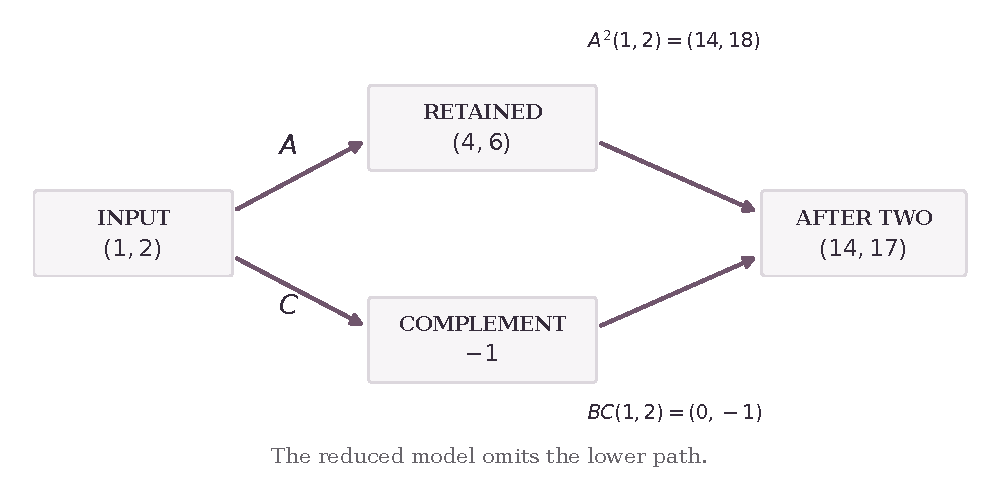
\includegraphics[width=\linewidth]{return_paths.pdf}
\caption{Two paths contribute to the second retained observation. The direct path stays in the retained space. The other leaves and returns. The labels are the exact values for the rational example in the text.}
\label{fig:return}
\end{figure}

\FloatBarrier
\subsection{From a calculation to a reusable law}

The general packet formulation uses a finite family of pairwise annihilating projectors whose sum is the identity. Write \(T_{ij}=P_iTP_j\). Then
\[
T=\sum_{i,j}T_{ij},
\qquad
(ST)_{ik}=\sum_j S_{ij}T_{jk}.
\]
Composition follows paths through intermediate packets. The laws are familiar block algebra. Their methodological value is that they provide an exact interface for tracking what a decomposition retains and what it omits. Realization Calculus uses such interfaces to organize more specialized constructions without pretending that an arithmetic lane and an analytic subspace have identical additional properties.\sourceref{rc}

The example also suggests a better experiment. Merely repeating the first retained observation does not challenge the simplification. Continuing the system does. More generally, a test should be designed to expose the information a representation discards. That may mean increasing the number of compositions, changing a boundary condition, or testing a component that a cancellation had concealed.

Invariance supplies a sufficient answer in this setting. If \(QTP=0\), then \(T\) never sends a retained input into the complementary space, so the retained space is invariant and repeated restriction is exact. The condition is stronger than vanishing on one selected input. It is also stronger than the disappearance of one particular return term. A method that records the operator and its domain can distinguish these statements instead of treating them as interchangeable successes.

\clearpage
\subsection{The missing coordinate becomes memory}

The discrepancy can do more than refute a simplification. It can tell us how to construct an exact replacement. Write a general block evolution as
\[
 u_{n+1}=Au_n+Bv_n,\qquad v_{n+1}=Cu_n+Ev_n,
\]
where \(u_n\) is retained and \(v_n\) is complementary. Suppose first that \(v_0=0\). Repeated substitution in the second equation gives
\[
 v_n=\sum_{j=0}^{n-1}E^{n-1-j}Cu_j.
\]
For \(n=0\) the sum is empty. The induction step multiplies the preceding sum by \(E\) and adds \(Cu_n\). Substituting into the first equation therefore proves, for every \(n\geq0\),
\begin{equation}\label{eq:memory}
 u_{n+1}=Au_n+\sum_{j=0}^{n-1}BE^{n-1-j}Cu_j.
\end{equation}
The reduced description is exact, but it now carries memory. In the displayed rational example \(E=2\), and the first correction is \(BCu_0=(0,-1)^{\mathsf T}\). Equation~\eqref{eq:memory} gives the correct second observation and governs every later step. This is a deduction from the block equations, not a fitted correction to a single failed experiment.

The requirement \(v_0=0\) is substantive. With a nonzero initial complementary state, the formula for \(v_n\) contains the additional term \(E^nv_0\), and the retained evolution contains \(BE^nv_0\). An unknown \(v_0\) cannot simply be erased. Either the problem supplies it, the retained data determine its relevant effect, or the prediction must preserve the remaining ambiguity.

The example now contains a complete research cycle. A proposed simplification fails. A transfer identity isolates the cause. Eliminating the hidden coordinate constructs a replacement. Induction proves the replacement for all times under stated initial data. Exact calculations can then test its implementation. The resulting memory formula is a reusable piece of mathematics. It may cost more to store a history than a single state, so an exact realization is not automatically the cheapest one. What has been gained is a clear account of the choice.

\clearpage
\subsection{Defects must be transported before they are combined}

A similar issue arises when comparing two sequences of transformations. Let \(T:X\to Y\) and \(S:Y\to Z\) be linear maps, with comparison maps \(p:X\to X_0\), \(q:Y\to Y_0\), and \(r:Z\to Z_0\). Suppose \(T_0:X_0\to Y_0\) and \(S_0:Y_0\to Z_0\) are the proposed reduced maps. Their defects are
\[
\Delta_T=qT-T_0p,
\qquad
\Delta_S=rS-S_0q.
\]
Adding and subtracting \(S_0qT\) gives
\begin{equation}\label{eq:composition}
\Delta_{ST}=rST-S_0T_0p
=\Delta_S T+S_0\Delta_T.
\end{equation}
One defect is evaluated after \(T\). The other is carried forward by \(S_0\). Only then do they have the common source and target needed for addition.

This is what it means for a calculus to constrain its user. The phrase ``the errors add'' is not enough. The maps determine how they add. In another setting subtraction may not be defined at all, and an appropriate comparison must replace this formula. The shared method is the discipline of specifying the comparison, not the indiscriminate use of linear notation.

Accounting for a remainder does not require retaining every detail forever. It requires a reason why a discarded detail is irrelevant to the protected task, or a certificate of the effect it may still have. Once that reason is explicit, simplification can become both more aggressive and more trustworthy. The next step is to ask whether an identified defect can actually be removed.

\essaychapter{When failure becomes an obstruction}

A search that has found no solution has established something about the search. It has not necessarily established anything decisive about the existence of a solution. Perhaps the representation is poor, the search space too narrow, or the required idea absent. An obstruction analysis asks for more: a mathematical condition that every permitted solution must satisfy. A verified failure of that condition can certify nonexistence, rather than merely report an unsuccessful search.

The distinction is exact in a linear correction problem. Let \(D:U\to W\) be a linear map over a field, and let \(r\in W\) be a defect. An admissible correction is a vector \(h\in U\) satisfying \(Dh=-r\). Such a correction exists precisely when the class of \(r\) vanishes in the quotient
\[
W/\operatorname{im}D.
\]
Indeed, vanishing says \(r=Dg\) for some \(g\), so \(h=-g\) corrects it. Conversely, a correction puts \(r\) in the image. The quotient records exactly what the available corrections cannot change.

Take \(U=\mathbb Q\), \(W=\mathbb Q^2\), and \(D(u)=(u,u)\). Only diagonal corrections are allowed. For \(r=(1,2)\), the functional
\[
\lambda(w_1,w_2)=w_2-w_1
\]
vanishes on every possible correction but satisfies \(\lambda(r)=1\). If \(Dh=-r\) held, applying \(\lambda\) would give \(0=-1\). No additional search is needed. The functional is a short certificate of impossibility for the stated correction problem.

Now allow \(D'(u,v)=(u,u+v)\). The choice \((-1,-1)\) supplies the correction \((-1,-2)\), and the defect disappears. Nothing contradictory has happened. The admissible correction space has changed. That change may be an intelligent way to solve a broader problem, but it is not a solution of the original problem unless the extra freedom was permitted.

\subsection{A repair has to preserve something}

In a serious application, the restrictions are often the point. One may need to keep a boundary value, retain integrality, preserve positivity, or leave an already established observation unchanged. A method that removes every defect by discarding these requirements has not solved the task. It has replaced it.

For a linear protected quantity \(p:U\to V\), corrections that leave the quantity unchanged lie in \(\ker p\). The relevant correction image is therefore \(D(\ker p)\), not all of \(D(U)\). The obstruction must be calculated relative to that smaller image. This is the elementary form of protected repair developed in the realization framework. It explains why two superficially identical defects may have different answers when their preservation requirements differ.\sourceref{ks,ppt}

Even a valid obstruction test needs its logical direction stated. A nonzero test value may prove impossibility, while a zero value merely removes one known reason for failure. A complete criterion proves the converse as well. The linear quotient above is complete for its declared problem. A more complicated invariant should not inherit that completeness merely because we also call it an obstruction.

The same care applies to small residuals. On the Hilbert space \(\ell^2\), define \(D(x)_n=x_n/n\) for positive integers \(n\). The map is bounded and injective. For the unit vector \(e_n\), however,
\[
\|De_n\|=1/n\longrightarrow0,
\qquad
\operatorname{dist}(e_n,\ker D)=1.
\]
There is no uniform bound \(\operatorname{dist}(x,\ker D)\leq C\|Dx\|\) on this space. Taking \(x=e_n\) would require \(1\leq C/n\) for every \(n\). A tiny residual can therefore coexist with a fixed distance from the exact solution set. A stability estimate needs additional structure, not just a smaller numerical threshold.

This makes the word ``resolution'' demanding. A resolution may supply an admissible correction, a finer representation, or an estimate relating the defect to a genuine solution. It must say which of these it provides. Existence, a constructive algorithm, a canonical choice, and a stable numerical procedure are separate achievements, even when they concern the same equation.

Failure now has several possible outputs. A witness can close an existence problem. A separating functional can close a nonexistence problem. A reduction can isolate the one hypothesis still needed. The last is not equivalent to a solution, but it can substantially improve the next inquiry. Instead of returning to the original question with no guidance, the researcher returns with a sharply located boundary.

There is a practical reason to preserve this boundary. A later idea may enlarge the correction space legitimately, supply the missing stability estimate, or reveal that the requested preservation was unnecessary. The failed attempt then becomes reusable mathematics. Its value comes from the precision of what it leaves behind, not from failure considered as a virtue in itself.

\essaychapter{Experiment, conjecture, and proof}

Mathematical experimentation is most useful when it asks a question that competing explanations answer differently. More data are not automatically more insight. In the returning-coordinate example, the decisive experiment was not greater precision at the first step. It was a second step. The experiment succeeded because it challenged the assumption that the retained state was sufficient for continuation.

Exact computation is particularly valuable when the phenomenon itself is exact. Integer, rational, and finite-field arithmetic can distinguish a true cancellation from a small floating-point remainder. Symbolic manipulations can expose the invariant behind a numerical pattern. But exactness of the calculation and generality of the conclusion are different matters. A correct computation on finitely many inputs establishes those instances. To establish an unbounded statement, one still needs an argument covering the remaining cases, or a proved reduction showing that the finite cases are exhaustive.

The tradition of experimental mathematics has long treated computation as an instrument for discovering patterns, rejecting conjectures, and identifying routes to proof. Bailey and Borwein describe this active role explicitly. The Komorebi approach belongs in that tradition, while emphasizing the representation and obstruction structure carried from one experiment to the next.\sourceref{expmath}

\subsection{An arithmetic pattern with its mechanism exposed}

A small generating-function calculation illustrates the movement from pattern to explanation. Define the signed Euler numbers by the formal power series identity over \(\mathbb Q\),
\[
F(t)=\operatorname{sech}t=\sum_{n\geq0}E_n\frac{t^n}{n!}.
\]
The initial coefficients are \(1,0,-1,0,5,0,-61,0,1385\). Multiplication by \(e^t\) gives transformed coefficients
\[
b_n=\sum_{k=0}^n\binom nk E_k.
\]
Their initial values are \(1,1,0,-2,0,16,0,-272,0\). A finite computation suggests that every positive even index has disappeared. The reason is not hidden in the numerical list:
\[
e^t\operatorname{sech}t
=\frac{\cosh t+\sinh t}{\cosh t}
=1+\tanh t.
\]
The series \(\tanh t\) is odd. Thus \(b_{2j}=0\) for every \(j\geq1\). Multiplication by \(e^{-t}\) recovers the original coefficients, so the disappearance is a reorganization of information, not the destruction of the sequence.

The calculation does not prove a prime-power divisibility theorem. It establishes a parity statement through an invertible change of realization. A valuation claim would require a further arithmetic argument. This is an instructive boundary: a useful identity can be both completely proved and insufficient for the next conjecture.

Residue selectors make the mechanism more general. Let \(F(t)=\sum_{n\geq0}a_nt^n\) be a formal series over \(\mathbb C\), let \(\zeta\) be a primitive \(m\)-th root of unity, and choose \(0\leq r<m\). Then
\[
\frac1m\sum_{j=0}^{m-1}\zeta^{-rj}F(\zeta^jt)
=\sum_{n\equiv r\;({\rm mod}\,m)}a_nt^n.
\]
For the coefficient of \(t^n\), the multiplier is the average of \(\zeta^{j(n-r)}\). It is one when \(m\) divides \(n-r\), and zero otherwise by the finite geometric-sum identity. The filter selects a lane of coefficients exactly. Because the argument is coefficientwise, it needs no analytic convergence assumption.

This is also where changing the coefficient setting matters. The displayed average uses roots of unity and division by \(m\). Transporting it into an integral or \(p\)-adic argument requires control of those operations, especially when \(p\) divides \(m\). A valid identity over \(\mathbb C\) does not by itself supply the integral estimate one hopes to extract from it.

\subsection{Let the experiment challenge the explanation}

A productive experiment records the exact input, the proposed rule, and the observation that could separate it from an alternative. In arithmetic, this may mean moving beyond the first nonzero valuation, changing a residue class, or testing the boundary index where a conjectured formula begins. In an operator problem, it may mean composing once more or changing the protected subspace. The design follows the suspected failure mechanism.

Positive and negative cases both belong in the record. An example outside the hypotheses can explain why a hypothesis is needed. A degenerate example can reveal that a program is silently dividing by zero. An independent calculation can detect an indexing error that a symbolic derivation inherited from its own input. These are different kinds of evidence, and their usefulness depends on preserving the difference.

The resulting loop is not simply calculation followed by proof. A calculation suggests a structure. A counterexample refines it. A proof identifies why the structure works. New tests then challenge the implementation and the translation of the proof back into the original problem. Each stage asks the others a more precise question. Formal verification becomes valuable at exactly this interface.

\essaychapter{The discipline of checking}

The phrase ``the proof was checked'' leaves an important question open. Was the argument reviewed, a calculation reproduced, a formal derivation accepted, or a software package tested? Each check has a particular scope. Their relationship needs to be established.

Lean gives a particularly strong form of deductive checking. Its kernel checks a proof of a formal statement relative to the definitions, theorems, and axioms in the environment. Lean's own validation guidance distinguishes this question from the meaning of the theorem statement, and describes additional checks for axiom dependencies and stored proof artifacts.\sourceref{leanvalidation}

The formal declaration is the proposition established, not a label attached to a prose claim. Its quantifiers, domains, coercions, and hypotheses must match the intended mathematics. A theorem about a fixed finite model does not cover every model. Assuming an extension exists does not construct it. These distinctions determine what the proof actually gives us.

Formalization makes these distinctions productive. Writing the statement can expose an ambiguity. Supplying an actual map can reveal where an argument relied on resemblance. A proof obligation that remains open can isolate the missing theorem more precisely than confident prose.

\subsection{Acceptance is not the whole policy}

Axioms require a separate audit. Lean permits new axioms and records proof dependencies. Postulating \(\mathrm{False}\) allows any proposition to be derived. The derivation is valid relative to that assumption. A project that disallows the assumption must reject the dependency.\sourceref{leanaxioms}

A useful audit therefore follows dependencies transitively. Looking only for a placeholder in the final theorem can miss one in an imported lemma. The commonly admitted mathematical basis in Lean includes \texttt{propext}, \texttt{Classical.choice}, and \texttt{Quot.sound}. A result using only an allowed subset has passed an axiom-policy check, not an automatic test of every intended application.\sourceref{leanaxioms,leancommunity}

Ordinary hypotheses are different from global axioms. The implication \(\mathrm{False}\Rightarrow P\) needs no newly postulated axiom, yet cannot establish \(P\) without the impossible premise. Less conspicuous hypotheses can conceal the same application gap. The review must therefore inspect the theorem's quantifiers and show that the required data are available where the result is used. A legitimate conditional theorem need not supply every application itself. Its conditional scope must remain visible.

The project record offers a concrete illustration. The verification section of \emph{Proof-Path Theory} describes deliberately invalid equalities, witnesses, and conjunction models, as well as a proof placeholder. It also describes an explicit false axiom whose consequence Lean accepts, while a separate project policy rejects the dependency. The report distinguishes replay through Lean's own kernel from an independent implementation, and identifies the reused external dependency cache. These are scoped records, not a blanket claim that every page of the research program has received the same check.\sourceref{ppt}

A negative control should fail for the intended reason. If a false equality is never checked because the file cannot import its dependencies, the test has not demonstrated mathematical rejection. A timeout is similarly inconclusive. This makes diagnostics part of the evidence. The useful record says which proposition or witness was rejected, by which check, and under what environment.

The principle extends beyond Lean. A certificate checker should reject corrupted witnesses. A manifest validator should detect altered files. A parser should reject malformed records rather than assign reassuring defaults. These tests address distinct ways a claim can become disconnected from its evidence.

\subsection{Reproduction binds the claim to an artifact}

A proof lives in a source tree, a toolchain, and an imported environment. The Lean community's verification guidance therefore asks whether the project builds, whether the relevant theorem file is actually included, which axioms it uses, and whether its statement expresses the advertised claim. A source listing that looks plausible is not a completed verification record.\sourceref{leancommunity}

Pinned dependencies, source digests, build commands, and preserved logs make this record recoverable. A digest identifies bytes. It does not prove that the bytes contain correct mathematics. A successful replay checks a particular artifact under a particular environment. Repeating the same kernel check can demonstrate reproducibility, but does not turn that kernel into an independent checker. An alternate proof or independently implemented validator may challenge a different class of failure.

Semantic review belongs alongside mechanical checks. Compare the formal theorem with the prose claim. Instantiate its hypotheses on meaningful examples. Map the manuscript result to the declarations establishing it, rather than relying on suggestive names. The aim is not paperwork, but an inspectable relationship between a claim and its evidence.

More tests help when they cover new failure modes. Repetition does not remove a shared mistaken definition. Conversely, a short proof checked under a clearly stated basis can deserve strong confidence. Precise qualification should sharpen that confidence, not turn established results into perpetual uncertainty.

Verification thus changes discovery by making statements precise and exposing missing interfaces. It tells the next inquiry what has survived. The certificate records that achievement, while the surrounding path may still carry useful mathematics.

\essaychapter{The field surrounding a proof}

Suppose a theorem has two proofs. One is short and efficient to verify. The other introduces a construction useful for a nearby problem. The first may be preferable for certification, while discarding the second may damage further inquiry. The two tasks value different information.

Proof-Path Theory makes this distinction explicit. A proof certificate is a selected derivation of a target from admitted premises. The surrounding proof field is a larger typed collection of claims, justifications, evidence, and alternatives. A recorded counterexample is not promoted into a proof step. A conjectured transition is not treated as certified because it appears beside a theorem. Status and scope belong to the record.\sourceref{ppt}

The finite model uses justification hypergraphs because ordinary arrows can hide an important distinction. A step may require both \(A\) and \(B\) to obtain \(L\). Another conclusion may have two independent routes, either of which is sufficient. The former is a conjunction of premises. The latter is an alternative between justifications. A faithful record must preserve which kind of dependency is present.

For example, take certified steps \(\{A,B\}\Rightarrow L\) and \(L\Rightarrow T\). They form one certificate for the target \(T\). A second route might use \(A\Rightarrow M\) and \(\{M,B\}\Rightarrow T\). A candidate extension from \(M\) to a new target \(U\) can remain visible without becoming part of either certificate. It may be valuable precisely because it suggests what to investigate next, but its value does not make it valid.

\begin{figure}[htbp]
\centering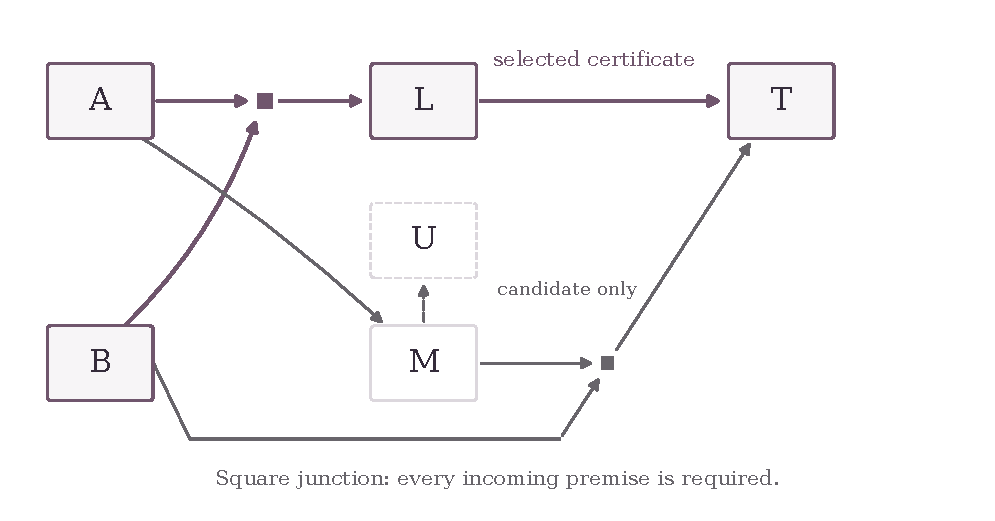
\includegraphics[width=\linewidth]{proof_field.pdf}
\caption{A declared proof field and one selected certificate. Small square junctions mean that all incoming premises are required. Solid alternative edges are certified but unselected. The dashed extension is a candidate and cannot certify its target. Line crossings are not junctions.}
\label{fig:field}
\end{figure}

\subsection{Compression depends on the next question}

The final proof is a useful compression. It removes material unnecessary for establishing the endpoint. But sufficiency for endpoint verification does not imply sufficiency for teaching, semantic audit, or further discovery. This is the same factorization issue encountered earlier: a retained record may answer one family of questions while merging distinctions another family needs.\sourceref{ppt}

A later task may require a discarded construction. Recovery may mean rereading a source, rerunning a computation, or repeating a search. When future tasks and their weights are specified, retention can be compared with this expected reconstruction cost. The comparison is relative to that model, not a universal measure of mathematical importance.

This suggests selective preservation rather than indiscriminate accumulation. Keep the example that explains a necessary hypothesis. Keep the obstruction that rules out a broad family of approaches. Keep a reusable comparison map and the test that caught an important translation error. A thousand nearly identical failed calculations may be less useful than one concise account of the reason they fail.

Revision also changes the record. Strengthening a lemma's hypothesis can affect every later argument that uses it. Those descendants need review, but are not automatically false. Some may already satisfy the stronger hypothesis. Others may have alternate proofs. A dependency record identifies where to look, allowing correction to propagate without treating the entire development as either untouched or destroyed.\sourceref{ppt}

The proof field is a declared mathematical record, not a recovery of every thought that produced a theorem. Its selection and provenance should remain visible. Dependencies extracted from Lean describe the artifact, but cannot reconstruct unrecorded experiments or every choice preceding it.\sourceref{ppt}

Review has a similar dependence problem. Two assessments can share the same mistaken definition or the same unexamined example. Agreement then provides less new information than agreement between genuinely different checks. Proof-Path Theory studies explicit models of such dependence. Their methodological lesson is to ask what a review adds, not to infer the motives or competence of particular reviewers from a model.\sourceref{ppt}

A mathematical archive becomes powerful when it can answer both ``why does this follow?'' and ``what can we do next?'' The certificate addresses the first question. The richer field can help with the second. Preserving both is especially consequential when the next researcher is not the same person, or not the same kind of reasoner.

\essaychapter{Human and machine in one research process}

A human and a machine can participate in the same inquiry without performing identical roles. Either may suggest a representation, locate an analogy, or expose an inconsistency. A formal checker performs a different task from both: it evaluates a precisely encoded derivation under its rules. The collaboration becomes useful when these contributions can be connected without confusing their authority.

The essential separation is between generating a candidate and establishing its status. An idea can be worth pursuing before there is evidence that it is true. A machine may propose many such ideas, and a human may recognize which ones bear on the real difficulty. The direction of assistance can also reverse. What matters is that the resulting claim eventually confronts the same mathematical requirements, regardless of who first proposed it.

Realization Calculus suggests a way to make that confrontation less dependent on persuasive prose. A candidate transformation can declare its input and output types, the questions it preserves, and the defects it introduces. A proposed repair can state its correction space and protected data. A proof obligation can specify which of these assertions has not been established. The object passed between collaborators is then more than an answer. It contains the conditions under which the answer could be used.

There is a substantial possibility here. If a reasoning system can inspect these objects, it can search for a missing comparison map rather than restart an entire problem. It can reuse a proved correction principle where the required hypotheses match. It can recognize that a failed experiment has isolated a narrower question. This is a route toward machine-suited mathematics whose operations remain mathematically legible.

That route does not demand unfamiliar mathematics merely for the sake of unfamiliarity. Reconstructing a classical result in a shared calculus can demonstrate that the language preserves the intended structure and supports reuse. New results within the same language test its capacity to go further. These are complementary contributions. Whether a particular theorem is historically new remains a question about that theorem and its relation to prior work, not about the novelty of every symbol used to state it.

\subsection{The rate of proposal and the rate of checking}

The practical danger is not simply that a machine may be wrong. Any collaborator may be wrong. The danger is that the production of plausible claims can outpace the work needed to inspect them. If candidate arguments accumulate faster than their definitions, dependencies, and evidence can be checked, a research program can become larger without becoming more reliable.

A disciplined workflow therefore limits what unverified material is allowed to support. Candidate results may guide exploration, but they do not silently become certified premises. The current research state should make the next unresolved obligation visible. After a substantial revision, the applicable tests and dependent arguments should be revisited. A continuation record should identify an actual restart point rather than merely report that much progress has been made.

This discipline also protects continuity. A new session, a different collaborator, or an external reader should not have to infer the accepted statement from a long conversation. The source artifact, claim map, and scoped evidence should carry that responsibility. Reproducible Python calculations, formal sources, explanatory manuscripts, and visual accounts can provide different views of the same work, provided the correspondences among them are maintained.

For the running example, the durable record is short but specific. The task is to reproduce retained observations of the full evolution from the declared initial state. The failed candidate is iteration of \(A\) alone. The counterexample occurs at the second observation. The replacement is the memory law, with its initial-state hypothesis and induction proof. A later researcher can now change the question intelligently: ask for a shorter memory, a bound on a truncated history, or a sufficient statistic that can be updated cheaply. Keeping only the final matrix product would conceal this direction of inquiry.

An inspectable grammar is not a promise that every problem becomes easy, or that every missing realization can be generated from a finite menu. It is a way to make many important operations composable. Its strength should appear in the quality of those compositions: fewer hidden changes of meaning, more useful reusable components, and sharper accounts of what fails.

Human judgment is not removed from such a process. Choosing a question, recognizing significance, and deciding which representation deserves investigation remain consequential. Nor is machine contribution reduced to transcription. Exploration, construction, formalization, and criticism can all materially change the mathematics. The method should make those changes available for examination rather than resolve the collaboration through a story about which participant deserves all the intelligence.

The strongest account of the work is therefore carried by its artifacts. What was constructed? What was proved? Which incorrect route was rejected, and why? Which result can another researcher now use? Those questions provide a basis for discussing both mathematical achievement and the effectiveness of the collaboration without relying on the volume of generated text as evidence of either.

\essaychapter{A scientific method for mathematics?}

There is a serious sense in which this is a scientific method for mathematical inquiry. It begins with questions, forms candidate explanations, designs discriminating tests, records failure, revises representations, and demands evidence that can be inspected by someone other than the discoverer. It also requires a limit on the analogy. The final justification of an abstract theorem is not the same kind of achievement as the experimental confirmation of a physical model.

For a universal mathematical claim, a valid counterexample is decisive. Successful tests on many inputs are not generally decisive in the opposite direction. They may justify further investigation or reveal the correct statement, but they do not supply the missing universal deduction. A computation can nevertheless be a complete proof of a finite claim, and a finite computation can complete an unbounded theorem when a proved reduction makes it exhaustive. The relevant distinction is logical coverage, not whether a computer was used.

\subsection{An existing conversation, a particular synthesis}

P\'olya's \emph{How to Solve It} places the activity of finding a solution beside the presentation of a finished one. Its questions encourage the solver to understand the task, seek related problems, examine a plan, and reconsider the result. The heuristic tradition is already concerned with making discovery teachable without pretending that useful advice guarantees success.\sourceref{polya}

Lakatos's \emph{Proofs and Refutations} studies how conjectures and proposed proofs develop under criticism. Counterexamples can expose weaknesses in a statement or in the concepts used to formulate it, making revision part of mathematical development rather than merely an interruption. This provides an important precedent for treating failed arguments as sources of sharper mathematics.\sourceref{lakatos}

Experimental mathematics contributes methods for turning computation into an active instrument of inquiry. Formal verification contributes an exact language in which specified claims can be checked. Neither practice is invented by Komorebi. The methodological proposal is to connect them to a mathematical account of realization, preservation, obstruction, repair, and the retained field surrounding a proof.\sourceref{expmath,leanvalidation}

The contribution should be assessed at these connections. Does a change of realization carry a proved interpretation? Does the obstruction identify the exact admissible correction problem? Does a refinement preserve the original task? Can a certificate be traced to the statement in the manuscript? Does the archive preserve a construction another inquiry can actually use? A shared vocabulary matters when it makes these connections easier to establish and harder to fake.

The intended gain is cumulative. A correction lemma proved for a specified class of maps becomes available wherever that class is realized. A preserved obstruction rules out the same inadmissible repair in another setting. A formal correspondence prevents a translation from silently changing the target. These are concrete ways in which one inquiry can reduce the work of the next. The methodology asks that this transfer be exhibited, not merely described as unification.

There is no need to present the synthesis as a replacement for the rest of mathematics. A calculus earns its place by organizing relationships productively. Classical reconstructions can demonstrate breadth and coherence. New theorems, sharper reductions, and informative impossibility results can demonstrate further reach. The methodological argument is strongest when both are visible and neither is mistaken for the other.

\begin{figure}[htbp]
\centering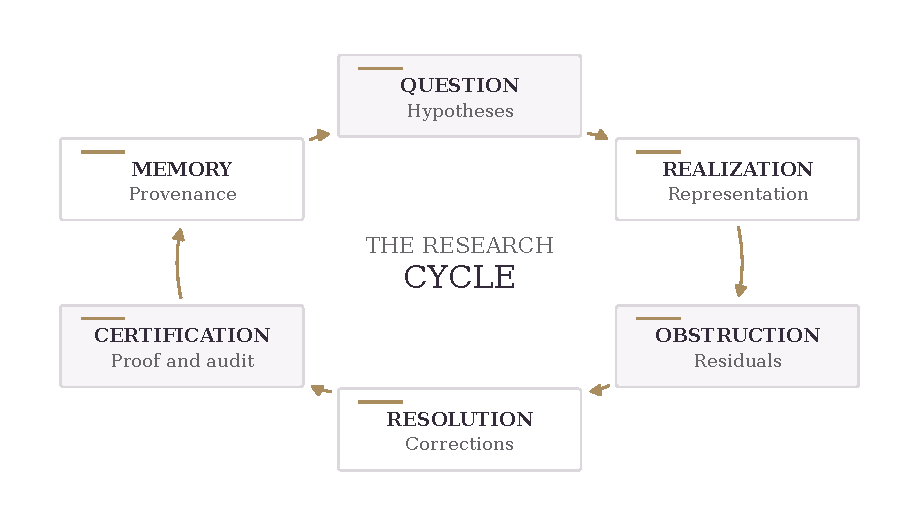
\includegraphics[width=.91\linewidth]{inquiry_cycle.pdf}
\caption{A research cycle, not an automatic theorem-producing pipeline. A candidate realization can lead to a construction, an obstruction, or a revised question. Certification governs which claims may enter the reusable mathematical record.}
\label{fig:cycle}
\end{figure}

\subsection{The method must also be answerable to evidence}

Whether this workflow improves mathematical research is itself a testable question. The validity of the displayed identities does not answer it. Neither does the existence of a substantial research collection. Those establish ingredients and examples. A claim of practical advantage requires a comparison designed to reveal both benefits and costs.

A credible evaluation would declare its tasks before selecting successes. One comparison could give two groups the same tools, starting material, and resource budget. One group would retain its ordinary working notes. The other would also maintain explicit realization contracts, scoped evidence, and the key failed obligations. Both would then receive a related task whose protected observation or admissible correction has changed. The prediction is specific: the structured record should help researchers identify which old results still apply and which must be revised.

Time spent creating and auditing that record belongs in the cost, not outside it. Tasks should include cases where a conventional method is already efficient. Independent reviewers should assess the resulting claims without being told which workflow produced them. Assignment and order should be controlled where practicable, and failed attempts should remain visible. A further comparison could retain the same source material but remove its dependency links, testing whether the organization adds value beyond simply keeping more notes.

The evaluation should count distinct outcomes separately. A completed theorem, a valid counterexample, and a proved reduction to an unresolved obligation have different meanings. Timeouts are unresolved cases, not zero-cost successes or invisible exclusions. Verification time, source recovery effort, incorrect claims admitted, and useful components transferred to later tasks also matter. An approach that produces fewer proposals but more independently usable results may be better than one that fills an archive rapidly. An approach that adds administrative burden without improving discovery or reliability may be worse.

Independent checking should include the statement, not only the proof file. Failed attempts should remain in the sample. Reused lemmas should be credited for the work they save without counting the same lemma as a new discovery each time. A small successful study would support a claim about its task family, not about all mathematics. The protocol should be capable of showing that some parts of the methodology help and others do not.

This is the point at which the scientific analogy becomes strongest. The method contains mathematical components that can be proved sound within explicit hypotheses, and practical claims that can be tested against alternatives. Those two forms of accountability reinforce one another. A sound calculus with poor search procedures may be difficult to use. An efficient search procedure without reliable certification may produce little durable knowledge.

The proposal is therefore not a single recipe imposed on all discovery. It is a discipline for exposing the objects, choices, and obligations through which discovery proceeds. It asks that successful transformations become reusable mathematics and that unsuccessful ones leave more than an anecdote. Its ambition is to make discoveries accumulate as usable structure, rather than only as isolated answers.

\clearpage
\phantomsection
\section*{What the method leaves behind}
\addcontentsline{toc}{section}{What the method leaves behind}

Return to the finished proof. Its definitions now arrive in the right order. The decisive lemma appears exactly where it is needed. Nothing in this essay asks that the reader be forced to relive every false start. The clarity of the certificate remains an achievement.

What changes is what may stand beside it. There can be a record of the representation that made the theorem accessible, the invariant that survived a transfer, and the obstruction that defeated a plausible alternative. There can be an exact calculation that explains a hypothesis, a formal declaration that makes the conclusion inspectable, and a dependency record that tells a later researcher what a revision affects.

These objects do not all establish the same thing. Their separation is part of their usefulness. A conjecture can remain visible without borrowing the authority of a proof. A computation can be exact without claiming unbounded coverage. A conditional theorem can be powerful without pretending to supply its own hypotheses. A negative result can close a genuine question and redirect the next inquiry.

The methodological opportunity is to make these distinctions productive. A change of realization can turn an opaque problem into an algebraic one. A residual can show where information returns, and an exact memory law can turn that finding into a constructive replacement. An obstruction can identify why no admissible correction exists. A verified transformation can become a component in another proof. A preserved discovery field can allow a different mind to continue without reconstructing the whole inquiry from its final sentence.

This is a demanding conception of mathematical research, but not an austere one. It leaves room for intuition, speculation, surprise, and an idea whose value is not initially clear. What it refuses is the silent conversion of those possibilities into established facts. Creativity proposes what may be possible. The mathematics determines which proposal survives and under what conditions.

The Komorebi Methodology should be judged by that survival and by what becomes possible afterward. Its promise lies in results that can be reused, failures that sharpen the next question, and records that make correction easier rather than more costly. A method that makes such progress visible has done something substantial even before its broadest ambitions are settled.

The aim is not to automate the judgment of mathematics. It is to make more of mathematical discovery available to judgment.

\clearpage
\phantomsection
\section*{Sources and verification scope}
\addcontentsline{toc}{section}{Sources and verification scope}

\subsection*{The mathematical sources}
The realization discussion draws on the companion works listed below. \emph{Komorebi Realization Calculus} supplies the packet, transfer, and defect language. \emph{Komorebi Space} develops coherent views, protected repair, and the distinctions among existence, uniqueness, and stability. \emph{Proof-Path Theory} supplies the certificate and discovery-field distinction, together with its finite models of preservation, provenance, and review. References to recorded verification describe the source reports, not a new replay of those projects.

The elementary calculations in this essay are proved in the text. They illustrate the method and are not presented as new discoveries. The factorization criterion is a set-theoretic statement. The continuation criterion follows from factorization. The return, memory, and defect identities are linear statements. The memory formula retains the declared initial complementary state, including its extra contribution when that state is nonzero. The correction alternative is relative to the specified correction image. The finite-prefix example uses inclusion maps, and the stability example uses the stated bounded operator on \(\ell^2\). The roots-of-unity identity is coefficientwise over \(\mathbb C[[t]]\). Keeping these settings explicit is part of the argument.

\subsection*{What the accompanying checks establish}
The source package includes exact Python checks for the finite examples, the reconstructed memory evolution, coefficient calculations, small matrix identities, and the declared proof-field illustration. It includes deliberate invalid witnesses and false finite claims that those checks must reject. The mathematical tests use exact integer and rational arithmetic. Separate archive tests exercise the integrity validator on empty, incomplete, altered, and malformed records. They corroborate the displayed instances and the implementation, not a universal claim about mathematical discovery.

The proofs concerning an unbounded tower and an infinite Hilbert space are written arguments. Finite tests cannot replace them. No new Lean compilation of the essay or fresh audit of the wider Komorebi corpus is asserted. The accompanying audit record distinguishes calculation checks, source consultation, typesetting, and rendered-page review.

\subsection*{Historical placement}
P\'olya, Lakatos, and experimental mathematics provide intellectual precedents. The Lean sources support the discussion of formal checking. The comparison of research workflows remains a proposed study, not a completed experiment.

\clearpage
\phantomsection
\addcontentsline{toc}{section}{References}
\renewcommand{\refname}{References}
\begin{thebibliography}{9}
\setlength{\itemsep}{8pt}
\bibitem{rc} Komorebi P. \emph{Komorebi Realization Calculus}. Companion monograph essay. See ``Packets and the structure of transport,'' ``The permitted correction determines the answer,'' and ``The residual of a composite must be transported.''
\bibitem{ks} Komorebi P. \emph{Komorebi Space: Coherent Realizations, Obstructions, and Descent}. Companion mathematical monograph. See the preface, the chapters on views and protected correction, and the treatment of approximate answers and their limits.
\bibitem{ppt} Komorebi P. \emph{Proof-Path Theory: Certificates, Compression, Discovery Fields, and Mathematical Memory}. Companion mathematical paper. See Sections 2--4, 7--10, 15--17, and 24.6--24.7 for the specific formal record discussed here.
\bibitem{polya} G. P\'olya. \emph{How to Solve It: A New Aspect of Mathematical Method}. Princeton University Press, 1945. Second edition, 1957. See the prefaces and the discussion of the four phases, pp.~5--6. \href{https://sites.math.rutgers.edu/~zeilberg/math436/polya.pdf}{University-hosted scan}.
\bibitem{lakatos} Imre Lakatos. \emph{Proofs and Refutations: The Logic of Mathematical Discovery}. Edited by John Worrall and Elie Zahar. Cambridge University Press, 1976. \href{https://www.cambridge.org/core/books/proofs-and-refutations/575FC8A6B4FAB79E649EDF5FBB9C6E10}{doi:10.1017/CBO9781139171472}.
\bibitem{expmath} David H. Bailey and Jonathan M. Borwein. ``Experimental Mathematics: Examples, Methods and Implications.'' Author manuscript, 2005. See the introduction, pp.~1--2. \href{https://www.davidhbailey.com/dhbpapers/ams-expmath.pdf}{Author-hosted text}.
\bibitem{leanvalidation} Lean Project. \emph{The Lean Language Reference}, ``Validating a Lean Proof.'' \href{https://lean-lang.org/doc/reference/latest/ValidatingProofs/}{Official documentation}.
\bibitem{leanaxioms} Lean Project. \emph{The Lean Language Reference}, ``Axioms.'' \href{https://lean-lang.org/doc/reference/latest/Axioms/}{Official documentation}.
\bibitem{leancommunity} Lean Community. ``Did you prove it?'' Guidance on project builds, axiom dependencies, and theorem correspondence. \href{https://leanprover-community.github.io/did_you_prove_it.html}{Community verification guidance}.
\end{thebibliography}

\end{document}
